\section{Latihan}

Bisa karena biasa, rumit karena tak dicicil. Maka pemakaian git adalah masalah kebiasaan. Oleh karena itu, dalam pembukaan awal buku ini justru kita tidak dulu masuk kepada teori git tapi langsung praktek. setelah berkali-kali praktek maka akan timbul beberapa pertanyaan mengenai fungsi dari perintah-perintah git yang bisa dibaca pada bagian selanjutnya.


Skenarionya adalah kita akan melakukan kontribusi terhadap sebuah repo \textit{Open Source} di GitHub. Jadi latihan ini adalah latihan bagaimana ikut berkontribusi kepada repo \textit{Open Source} yang ada di Github yang selama ini digunakan oleh para relawan kode untuk bersama membangun kode program berbasis \textit{Open Source}.
\subsection{Konfigurasi Key}
Pertama kita masuk kepada tahapan \textit{setting} atau konfigurasi \textit{key} untuk mengakses semua repo dari \textit{profile} kita dari \textit{git bash}:

\begin{enumerate}
\item Buat akun di www.github.com terlebih dahulu
\item Install \textbf{Git Bash} dari alamat \textit{git-scm.com/downloads} di komputer Anda, kemudian buka \textit{git bash}.
\item Pastikan sudah ada di \textit{home directory} dengan mengetikkan perintah \verb|cd| kemudian \textit{enter}. Untuk mengetahui posisi Anda ada di direktori mana ketikkan perintah \verb|pwd| dan \textit{enter}.
\item \textbf{\textit{Generate Key}} dengan perintah listing \ref{lst:keygen}.

\begin{lstlisting}[caption=Perintah Membuat Key,label={lst:keygen}]
ssh-keygen -t rsa -b 4096 -C "your_email@example.com"
\end{lstlisting}
Hasilnya seperti yang terlihat pada gambar \ref{luaran1}.
\begin{figure}[!htbp]
\centerline{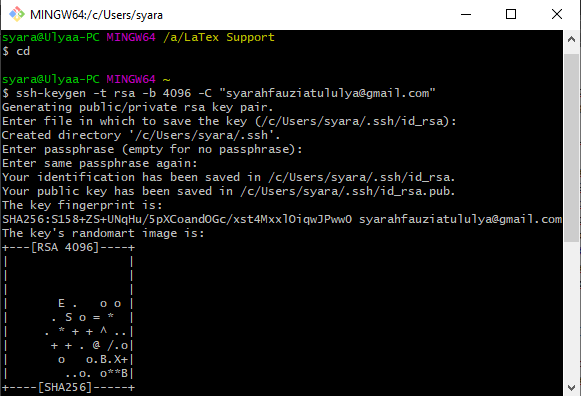
\includegraphics[width=.75\textwidth]{Figures/langkah1.PNG}}
\caption{Hasil Luaran 2}
\label{luaran1}
\end{figure}
\item Baca \textit{key} yang sudah di \textit{generate} dengan menggunakan perintah \ref{lst:catkey}.
\begin{lstlisting}[caption=Perintah Membaca Public Key,breaklines,label={lst:catkey}]
cat .ssh/id_rsa.pub
\end{lstlisting}
Hasilnya seperti pada gambar \ref{luaran2}.
\begin{figure}[!htbp]
\centerline{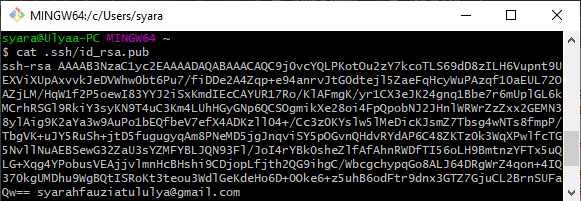
\includegraphics[width=.75\textwidth]{Figures/langkah2.PNG}}
\caption{Hasil Luaran 2}
\label{luaran2}
\end{figure}
\item Hasil luaran yang dibaca sebelumnya merupakan \textit{key} kita. Kemudian masukkan \textit{key} dengan masuk ke menu \textbf{\textit{Setting}} yang ada dipojok kanan atas, seperti pada gambar \ref{setting}. Lalu pada menu \textit{\textbf{SSH and GPG Keys}} tambahkan \textit{\textbf{New SSH key}} seperti pada gambar \ref{sshkeys}.
\begin{figure}[!htbp]
\centerline{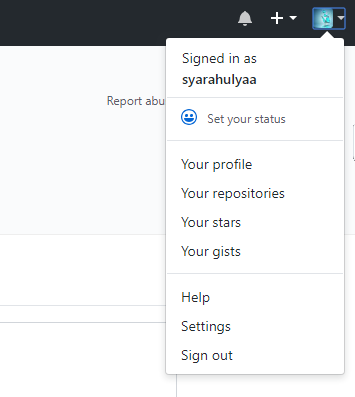
\includegraphics[width=.75\textwidth]{Figures/setting.PNG}}
\caption{Setting}
\label{setting}
\end{figure}
\begin{figure}[!htbp]
\centerline{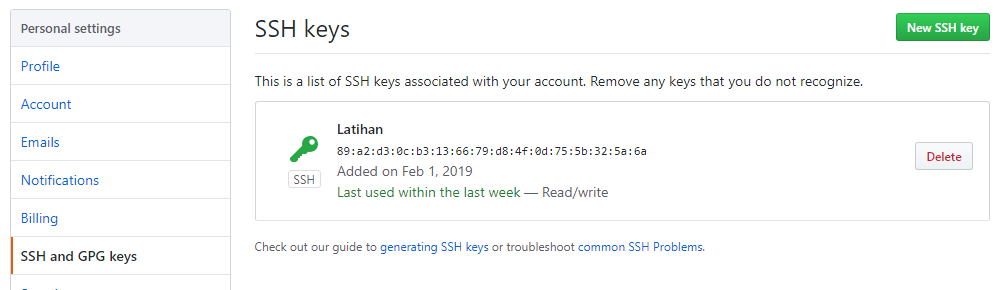
\includegraphics[width=.75\textwidth]{Figures/sshkeys}}
\caption{New SSH key}
\label{sshkeys}
\end{figure}
\end{enumerate}


\subsection{Fork Repositori}
Pertama kita cari repositori utama yang akan kita jadikan tempat berkontribusi dalam repositori tersebut. Jika sudah ketemu, kemudian klik Fork(Tombol kanan atas)seperti pada gambar \ref{fork}
  \begin{figure}[!htbp]
        \centering
            \includegraphics[width=.85\textwidth]{Figures/Click-Fork}
            \caption{Click-Fork}
        \label{fork}
    \end{figure}
yang dilanjutkan dengan memilih akun kita sebagai tujuan clone fork tersebut. Setelah selesai maka kita akan memiliki repo yang sama dengan repo yang anda fork. Contoh apabila anda melakukan Fork dari https://github.com/RepoAsal/Testing maka anda akan memiliki repo https://github.com/usernameAnda/Testing, dan kita akan bekerja pada repo hasil fork ini.


\subsection{Navigasi direktori dengan Git Bash}
Pertama kita tentukan terlebih dahulu folder tempat kita mengerjakan repo hasil fork kita. Misal di Drive D: folder Ganteng. Maka buka git bash kita dan arahkan menuju folder tersebut dengan perintah 
\verb|cd /D/Ganteng|.
Buka web repo fork kita di github klik tombol hijau \textbf{Clone or Download} pilih Clone with SSH(Gambar \ref{fig:clone1}) lalu salin kode yang tampak seperti \textit{git@github.com:usernameAnda/Testing.git}. 

\begin{figure}[!htbp]
\centerline{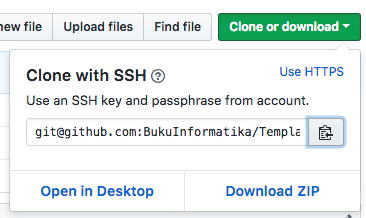
\includegraphics[width=.75\textwidth]{Figures/clone1}}
\caption{Hasil Perintah git clone}
\label{fig:clone1}
\end{figure}

Pada Git Bash ketik \textit{git clone git@github.com:usernameAnda/Testing.git} hasilnya seperti terlihat pada gambar \ref{gitclone}. 

\begin{figure}[!htbp]
\centerline{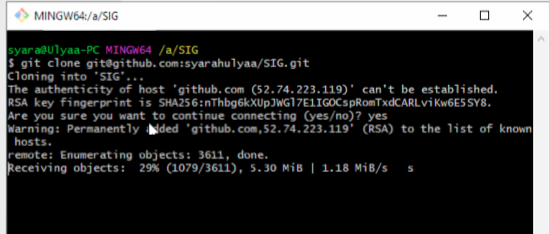
\includegraphics[width=.75\textwidth]{Figures/gitclone}}
\caption{Hasil Perintah git clone}
\label{gitclone}
\end{figure}

Setelah selesai, ketik perintah \textit{ls} maka akan muncul direktori baru yaitu folder Testing atau sesuai dengan nama repo Anda. masuk ke direktori tersebut dengan perintah \textit{cd Testing}. Kemudian ketik \textit{git status} akan muncul status dari repo git kita, ringkasan perintahnya bisa dilihat pada perintah listing \ref{lst:navigasikerepo}.sebagai contoh lihat hasilnya pada gambar \ref{lscdstatus}.

\begin{lstlisting}[caption=Navigasi direktori menuju repositori,label={lst:navigasikerepo}]
cd /D/Ganteng
git clone git@github.com:usernameAnda/Testing.git
ls 
cd Testing
git status
\end{lstlisting}

\begin{figure}[!htbp]
\centerline{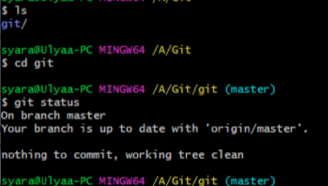
\includegraphics[width=.75\textwidth]{Figures/lscdstatus}}
\caption{Hasil Perintah ls, cd dan git status}
\label{lscdstatus}
\end{figure}

\subsection{Sinkronisasi dengan Repo Utama}

Karena ini repo hasil Fork maka kita harus selalu di sinkronisasi dari repo aslinya(tidak otomatis tersingkron). Sehingga perlu melakukan setting sumber repo tujuan yang merupakan repo asal. Pertama pastikan git bash sudah pada direktori repositori. Untuk melakukan sinkronisasi dengan repo asal kita harus mengeset satu kali dengan perintah listing \ref{lst:addupstream}.

\begin{lstlisting}[caption=Set Repo Asal Sebagai Upstream,label={lst:addupstream}]
git remote add upstream https://github.com/RepoAsal/Testing.git
\end{lstlisting}


Setelah melakukan \textit{setting} sekali di awal, kemudian selanjutnya kita tinggal melakukan sinkronisasi terus menerus sebelum melakukan perubahan dengan perintah listing \ref{lst:sinkronisasifork}.

\begin{lstlisting}[caption=Perintah Sinkronisasi dengan repo asal,label={lst:sinkronisasifork}]
git pull origin master
git fetch upstream
git pull upstream master
git push origin master
\end{lstlisting}


\subsection{Bekerja dengan Git Bash}
Sekarang kita mulai bekerja pada repo kita. Melakukan penambahan atau perubahan pada \textit{file}. Kemudian perubahan tersebut diminta untuk dimasukkan di repo utama tempat kita \textit{fork} repo kita. Urutan pekerjaan yang kita ulang terus menerus adalah sebagai berikut :
\begin{enumerate}

\item Sebelum mulai mengerjakan, sinkronisasi kembali dengan repo asli lagi agar terhindar dari konflik dengan perintah di listing \ref{lst:sinkronisasifork}.

\item Silahkan edit satu file yang akan di ubah atau ditambah lalu di simpan dan di tutup yang berada di direktori yang sudah disetting di navigasi direktori. Seperti terlihat pada gambar \ref{penanda}.
    \begin{figure}[!htbp]
        \centering
            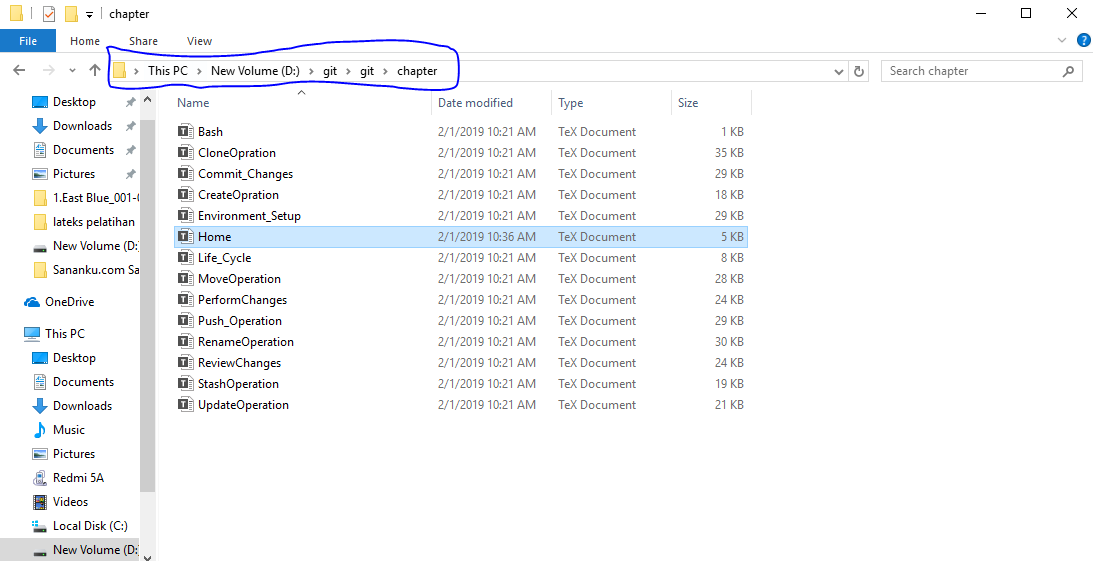
\includegraphics[width=.75\textwidth]{Figures/Capture}
            \caption{Direktori kerja git dari Explorer}
        \label{penanda}
    \end{figure}
\item Cek status git dengan perintah \textit{git status}, jika terdapat warna merah berarti belum kita add, jika terdapat warna hijau berarti belum kita commit.
\item File yang barusan diubah wajib kita daftarkan pada daftar perubahan yang kita lakukan yaitu dengan perintah \textit{git add namafilenya.tex}
\item Cek status git dengan perintah \textit{git status}, jika terdapat warna merah berarti belum kita add, jika terdapat warna hijau berarti belum kita commit.
\item Setelah file diubah maka kita wajib menambahkan komentar terhadap file yang kita ubah tersebut agar mempermudah kontributor yang lain mengetahui apa saja yang kita perbuat terhadap file yang sudah kita add. Perintah untuk memberi komentar dari file yang sudah di \textit{git add} adalah :\textit{git commit -m `perubahan apa yang telah kita lakukan di ceritakan di sini secara lengkap'}
\item Akan muncul permintaan konfigurasi global seperti gambar \ref{configglobal}. Maka kita harus memasukkan konfigurasi global dengan perintah \ref{lst:globalconfig}. Setelah itu kita ulang kembali perintah \textit{git commit}.
\begin{lstlisting}[caption=Perintah Sinkronisasi dengan repo asal,label={lst:globalconfig}]
git config --global user.email "awangga@gmail.com"
git config --global user.name "awangga"
git commit -m "perubahan apa yang telah kita lakukan di ceritakan di sini secara lengkap"
\end{lstlisting}
\begin{figure}[!htbp]
\centerline{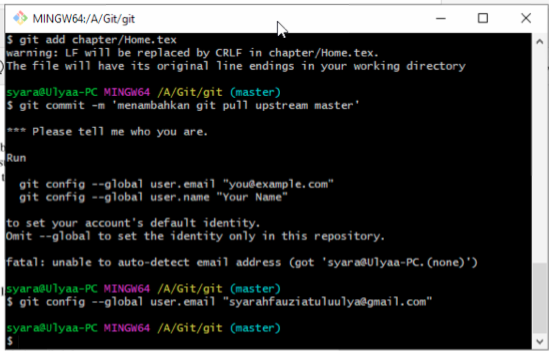
\includegraphics[width=.75\textwidth]{Figures/configglobal}}
\caption{Permintaan Setting Global}
\label{configglobal}
\end{figure}
Setting global ini hanya sekali saja ketika baru melakukan instalasi git bash, selanjutnya tidak akan muncul kembali permintaan setting global ini.

\item Cek status git dengan perintah \textit{git status}, jika terdapat warna merah berarti belum kita add, jika terdapat warna hijau berarti belum kita commit. Lihat gambar \ref{gitstatus}.
\item Kemudian file yang sudah kita ubah kita upload ke website github.com dengan perintah \textit{git push origin master}.
\item Sinkronisasi kembali dengan repo asli lagi sebelum beberapa detik melakukan \textbf{New pull request} agar terhindar dari konflik dengan perintah pada listing \ref{lst:sinkronisasifork}.
Apabila terdapat konflik jangan panik, itu namanya merge. Yang artinya menyatukan pekerjaan di web repo dengan repo lokal komputer kita. Apabila keluar tiba-tiba text editor dalam git-bash sehingga kita tidak bisa memasukkan perintah(tidak ada tanda dolarnya). Maka simpan saja dengan menekan tombol \textit{esc} kemudian ketik \textit{:wq} yang berfungsi untuk menyimpan dan tekan tombol \textit{enter}.

\item Buka web repo kita di website www.github.com
Contoh disini\\
 \textbf{https://github.com/usernameAnda/Testing} \\kemudian klik \textbf{New pull request}. Pastikan yang sebelah kiri atau base kita set kepada repo utama tempat fork kita yaitu RepoAsal/Testing dan compare pada sebelah kanan adalah repo kita, disini dicontohkan usernameAnda/Testing dan ilustrasi bisa dilihat di gambar \ref{pullrequest}. Klik tombol hijau \textit{Create Pull Request} kemudian teruskan sampai ada kembali tombol hijau yang kita klik lagi.
\begin{figure}[!htbp]
\centerline{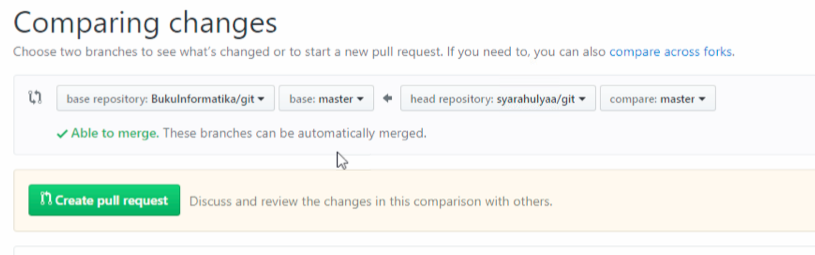
\includegraphics[width=.75\textwidth]{Figures/pullrequest}}
\caption{Setelah klik New pull request}
\label{pullrequest}
\end{figure}

\item Beritahukan admin repo utama untuk accept Pull Request Anda. Jika sudah di accept lakukan lagi langkah dari awal.
\end{enumerate}



\subsection{Mengatasi \textit{Error}}
Seorang programmer atau anak if pantang menyebutkan bahwa programnya error dan menyerah begitu saja. Error merupakan sebuah anugerah yang harus kita syukuri. Beruntungnya di git semua error memiliki petunjuk yang jelas. Sehingga apabila kita mendapati error, pastikan membaca dengan baik error nya dan selesaikan errornya dengan tenang dan santai. Karena error git sangat sederhana dan mudah sekali untuk diatasi. Atasi error tersebut dan jangan lari dari error tersebut.

\subsubsection{Kesalahan direktori}
Apabila bertemu error seperti pada listing \ref{lst:errorbukanrepo}. Pastikan git bash kita berada pada direktori repositori git yang dikerjakan, biasanya ditandai ada nama \textit{branch} di git bash nya. 

\begin{lstlisting}[caption=Kesalahan karena bukan pada direktori repositori,label={lst:errorbukanrepo}]
fatal: not a git repository (or any of the parent directories): .git
\end{lstlisting}

Sebagai contoh pada gambar \ref{configglobal} terlihat di ujung sebelum perintah dimasukkan ada tulisan \textit{master} warna biru muda. Itu artinya kita berada pada direktori repositori dengan \textit{branch} master. Di sebelah kiri \textit{master} ada tulisan kuning \textit{/A/Git/git}, yang artinya kita berada pada drive \textit{A:} windows. Pada drive \textit{A:} tersebut ada folder Git(G besar) yang didalam folder Git ada repo clone dengan folder git(g kecil). Posisi kita ada di dalam folder git tersebut.
Sebagai contoh kedua pada gambar \ref{penanda}, maka tulisan pada git bash tempat kita bekerja menjadi \textit{/D/git/git} atau \textit{/D/git/git/chapter}.

\subsubsection{Gagal Fetch Upstream}
Apabila anda pada saat melakukan \textit{git fetch upstream} atau \textit{git pull upstream master} keluar error seperti pada listing \ref{lst:errorfetchupstream}. 
\begin{lstlisting}[caption=Gagal melakukan fetch upstream,label={lst:errorfetchupstream}]
fatal: 'upstream' does not appear to be a git repository
fatal: Could not read from remote repository.

Please make sure you have the correct access rights
and the repository exists.
\end{lstlisting}
Maka ada dua kemungkinan, kemungkinan pertama anda belum melakukan set upstream seperti pada perindah di listing \ref{lst:addupstream}. Silahkan lakukan dahulu perintah di listing \ref{lst:addupstream}. Salah satu contoh repo yang belum melakukan perintah dari listing \ref{lst:addupstream} bisa dilihat di gambar \ref{errorfetch}.

\begin{figure}[!htbp]
\centerline{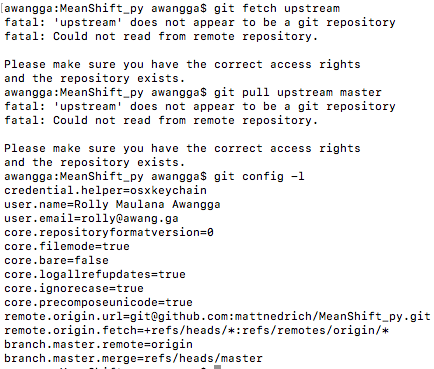
\includegraphics[width=.75\textwidth]{Figures/errorfetch}}
\caption{Gagal Fetch Upstream}
\label{errorfetch}
\end{figure}

Apabila anda sudah melakukan set upstream maka untuk melakukan pengecekan kita lihat dengan perintah di listing \ref{lst:gitconfig}.
\begin{lstlisting}[caption=Melihat konfigurasi git di repo komputer kita,label={lst:gitconfig}]
git config -l
\end{lstlisting}
Jika sudah ter set maka akan ada bagian yang berisi \textit{remote.upstream.url} seperti pada listing \ref{lst:upstreamconfig}.
\begin{lstlisting}[caption=Hasil perintah \textit{git config -l},label={lst:upstreamconfig}]
remote.upstream.url=https://github.com/RepoAsal/Testing.git
remote.upstream.fetch=+refs/heads/*:refs/remotes/upstream/*
\end{lstlisting}
Pastikan upstream berbentuk \textit{https} bukan \textit{ssh}. Apabila anda salah melakukan setting upstream anda bisa menghapusnya dengan perintah yang ada di listing \ref{lst:removeupstream}. Baru setelah itu lakukan lagi set upstream dengan perintah di listin \ref{lst:addupstream}.
\begin{lstlisting}[caption=Perintah menghapus upstream yang salah,label={lst:removeupstream}]
git remote remove upstream
\end{lstlisting}

\subsubsection{Salah Clone}
Buat pemula, kesalahan ini kadang terjadi jika tidak hati-hati membaca langkah-langkah sebelumnya. Apabila bertemu pesan kesalahan seperti pada listing \ref{lst:accessdenied}. Dari listing tersebut terliat \textit{jonluca/Anubis.git} adalah repo utama bukan repo clone kita perhatikan pada baris pertama listing to \textit{awangga} yang merupakan user github kita. Sehingga ini adalah kesalahan dalam clone, seharusnya repo yang di clone adalah awangga/Anubis.git. Ulang kembali kepada langkah clone repo, jika clone repo belum ada maka ulangi langkah fork.
\begin{lstlisting}[caption=Peringatan \textit{Permission denied},label={lst:accessdenied}]
ERROR: Permission to jonluca/Anubis.git denied to awangga.
fatal: Could not read from remote repository.

Please make sure you have the correct access rights
and the repository exists.
\end{lstlisting}



\subsubsection{Lupa langkah}
Sering-sering menggunakan git status untuk mengetahui sejauh mana kita melakukan perubahan. git status akan memberitahukan kita langkah apa saja yang harus kita lakukan, jika kita lupa langkah-langkah pengerjaan diatas. Pada gambar \ref{gitstatus}, jika terdapat warna merah berarti belum kita add, jika terdapat warna hijau berarti belum kita commit dan terakhir kita juga diberikan petunjuk untuk segera \textit{git push}.
\begin{figure}[!htbp]
\centerline{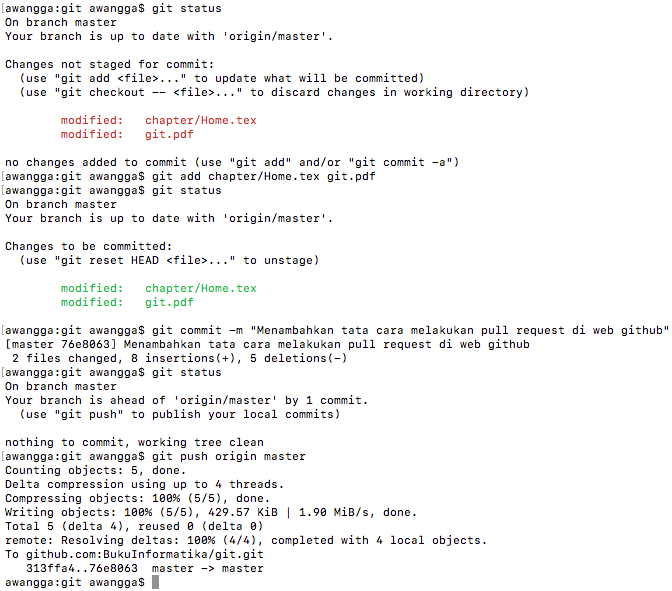
\includegraphics[width=.75\textwidth]{Figures/gitstatus}}
\caption{Berbagai macam luaran git status}
\label{gitstatus}
\end{figure}

\subsubsection{Konflik}
Ketiga, sebelum melakukan pekerjaan dan sebelum melakukan \textbf{New pull request}(dua kali). Pastikan repo lokal di komputer kita sinkron dengan yang ada di github baik itu repo asli maupun repo hasil fork milik kita dengan perintah pada listing \ref{lst:sinkronisasifork}. Apabila terdapat konflik jangan panik, itu namanya merge. Yang artinya menyatukan pekerjaan di web repo dengan repo lokal komputer kita. Apabila keluar tiba-tiba text editor dalam git-bash sehingga kita tidak bisa memasukkan perintah seperti pada gambar \ref{mergepull}. Maka simpan saja dengan menekan tombol \textit{esc} kemudian ketik \textit{:wq} yang berfungsi untuk menyimpan dan tekan tombol \textit{enter}.



\begin{figure}[!htbp]
\centerline{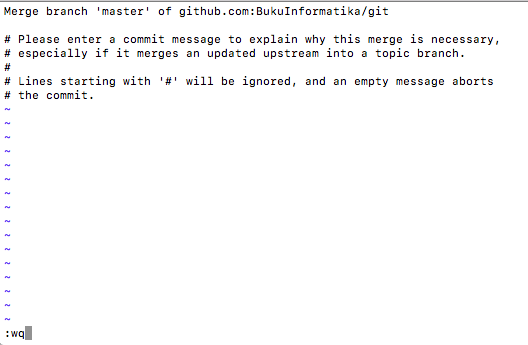
\includegraphics[width=.75\textwidth]{Figures/mergepull}}
\caption{Permintaan Merge dengan pesan standar yang keluar}
\label{mergepull}
\end{figure}
